\documentclass[12pt]{article}
%\usepackage[utf8]{inputenc}
\usepackage{amssymb,amsmath,graphicx,url,fullpage,amsfonts,verbatim,natbib}
\usepackage[small,bf]{caption}

% add bib to ToC
\usepackage{tocbibind}

\newcommand{\tatonnement}{t\^atonnement}

\input defs.tex

%\usepackage{spelling}
\usepackage[pdftex]{hyperref}

\title{Computing Market Equilibria via Convex Optimization}
\author{A.J. Friend \and Stephen Boyd}
\date{\today}

\begin{document}

\maketitle

\begin{abstract}

We consider the pure exchange market equilibrium problem of finding prices such
that the market clears, \ie, demand does not exceed supply. This is a classic
problem in economics, and has been discussed recently in the literature from a
computational complexity perspective. Indeed, depending on the utility
functions of the agents in the market, finding equilibrium prices can be
NP-hard. This paper will focus on the numerical computation of equilibria for a
subset of markets whose equilibrium problem can be cast as a convex program.
Recent advances in exponential cone solvers allow us to solve these problems as
conic programs. We will also introduce algorithms which scale to huge markets
and can be computed in a distributed fashion. We report numerical results for
huge random markets.

\end{abstract}

\newpage
\tableofcontents
\newpage

%todo santiago's stuff

\section{Introduction}
\subsection{Background}

We will consider exchange market equilibrium problems first introduced by
Walras in his in ``Elements of Pure Economics'' \cite{walras1896elements}.
Walras considers a market with agents trading goods with each other to selfishly
maximize their own utility functions. The market equilibrium problem is that of
finding prices for the goods such that the total demand of the agents does not
exceed the total amount of each good supplied by the agents for trade.

The market equilibrium problem has many applications, such as in (communication) network
congestion control \cite{kelly1997charging,srikant2004mathematics,
kelly1998rate,
low1999optimization,
yaiche2000game}, cloud computing \cite{gomes2012pure}, wireless spectrum management
\cite{ye2014competitive,vazirani2012notion},
and internet advertising \cite{vazirani2010spending}.

In full generality, Walras' model includes \emph{production}, \ie, processes by
which existing goods can be consumed to produce new goods which may enter the
market. We restrict this paper to the \emph{pure exchange} market, which allows for
trading of existing goods, but not production.

Walras suggested his natural \emph{\tatonnement{}} price adjustment scheme as a
means of computing equilibrium prices. However, the convergence of
\tatonnement{} and conditions for existence of equilibrium prices remained an
open problems for many years.

The Nobel Laureates Arrow and Debreu were the first to show that equilibrium
prices exist under mild conditions on the utility functions of agents
\cite{arrow1954existence}. However, these proofs relied on fixed-point theorems
(see \cite{border1989fixed})
and were initially non-constructive.
As such, they offered no practical means by which to compute these equilibria.

Later, Scarf and others 
\cite{scarf1967approximation,scarf1973computation,
scarf1982computation,eaves1972homotopies} were able to extend the fixed-point
ideas to produce path-following algorithms to compute equilibrium prices.
Unfortunately, however, these algorithms have exponential worst-case running times.

These initial results were followed by many new and varied computational
approaches to the market equilibrium problem.
Smale \cite{smale1976exchange,smale1976convergent} developed algorithms based
on Newton's method, but with no polynomial running time guarantees.
More recently, Esteban-Bravo has suggested techniques involving
interior point methods in a survey of computational techniques
for equilibrium problems \cite{esteban2004computing}.
Eaves \cite{eaves1976finite} showed that the problem could be cast and solved
as a complementarity problem \cite{isac1992complementarity}. The PATH
\cite{ferris2008path,ferris2000complementarity,ferris2000homotopy}
complementarity solver in GAMS \cite{rosenthal2004gams} is a popular tool for
solving equilibrium problems.
This short history of computational approaches is, of course, incomplete.
See \cite{codenotti2008experimental} and \cite{nisan2007algorithmic}
for more references.

This paper will investigate formulations of the market equilibrium problem as
convex optimization problems \cite{BoV:04}, which were rediscovered by Jain
\cite{jain2007polynomial}. This focus will restrict the types of markets we can
consider, but the convex optimization framework will allow us to solve these
problems efficiently, at scale, and with a variety of utility functions. The
original convex formulations for linear utility functions were stated by
Nenakov and Primak \cite{nenakov1983algorithm}. Jain's convex formulation was
later extended by Chen, Ye, and Zhang \cite{chen2007note,
chen2010equilibrium,ye2008path} to include some non-homogeneous utility
functions, and their proposed interior-point algorithms give the current
fastest polynomial-time complexity bounds for solving the market equilibrium
problem.

We will also consider an important special case of Walras' exchange market model,
which was first introduced by Fisher (see \cite{brainard2000compute}).
The Fisher model consists of agents endowed with
an initial amount of wealth which they use to purchase goods instead of trading
for them. Eisenberg and Gale \cite{eisenberg1959consensus, gale1960theory,
eisenberg1961aggregation} gave a convex program for finding equilibrium prices,
which we will use to handle a larger family of utility functions than in the
exchange case.

While there are large bodies of work across several disciplines covering the
economic interpretations, formulations, computational complexity, and
mathematical properties of these market equilibrium problems, this paper's
focus is on developing efficient computational techniques to solve
numerical instances of the given problems.
We provide two algorithmic approaches to the convex formulations
of these problems. The first is to capitalize on recently
developed exponential cone solvers \cite{scs} to provide a centralized
algorithm, easily solved within a convex modeling language, such as \cite{cvxpy,
cvx}. The second approach is to use the \emph{alternating direction method of
multipliers} (ADMM) \cite{boyd2011distributed} to produce a distributed and
scalable algorithm, allowing us to tackle huge problems.
As far as we are aware, the examples we solve are by far the largest
numerical examples reported in the literature.


\subsection{Outline}

In \S\ref{sec:defs}, we define two different \emph{market equilibrium problems}
(MEP) for the exchange and Fisher markets. The MEPs are defined by describing
the \emph{utility maximization problems} (UMP) of the agents in these markets,
and requiring that the solutions to the UMPs satisfy an equilibrium condition.

In \S\ref{sec:convex_form}, we convert the exchange and Fisher MEPs into two
different optimization \emph{formulations} which provide convex programs when
the utility functions satisfy certain properties (\S\ref{sec:util_funcs}). We
will refer to these specifically as the exchange and Fisher \emph{formulations}
to emphasize that a single \emph{problem} may be solvable using either
\emph{formulation}.

An exchange MEP must always be solved using the exchange formulation. However,
depending on the utility functions of the agents, Fisher MEPs can be solved
using the Fisher formulation, or by converting to an exchange problem and using
the exchange formulation. There are some Fisher MEPs which can only be solved
using the exchange formulation.

Once we have used one of the two formulations to state an MEP as a convex
optimization problem, we can write down the problem easily using a convex
modeling language and solve it with an appropriate centralized solver
(\S\ref{sec:centralized}). However, these methods will only scale up to
medium-sized problems. For large-scale problems, we will provide a distributed
algorithm in \S\ref{sec:distributed}. Luckily, the two convex formulations are
sufficiently similar that we can solve either one with this single distributed
algorithm.

We provide examples and convergence results for large random markets in
\S\ref{sec:examples}.


\section{Problem definitions}
\label{sec:defs}

In this section, we give precise definitions for the market equilibrium
problems that we will be studying. We define the exchange model, which deals
with agents trading initial endowments of goods to maximize their own utility
functions. A special case of the exchange model is Fisher model, where agents
start with some initial wealth, which they use to purchase goods  from a
globally available store.

Throughout the rest of the paper, $\reals^n_+$ will denote the nonnegative
real $n$-vectors, and $\reals^n_{++}$ will denote the positive real $n$-vectors.
Inequality symbols between two vectors of the same size, \eg, $x \leq y$,
will denote componentwise inequality. When it isn't ambiguous, $0$ may stand
in for a vector of any size whose elements are all zero.

Convexity and convex optimization will be used extensively. See \cite{BoV:04}
for a review.

\subsection{Utility function properties}

The convexity (and thus, solvability) of the optimization problems we are
interested in will depend on properties of the utility functions of the agents
in the market. To classify these functions, we state some simple definitions.

A function $u: \reals^n_+ \to \reals_+$ is \emph{homothetic} if for any $\alpha
> 0$ we have that $u(x) \geq u(y)$ if and only if $u(\alpha x) \geq u(\alpha
y)$. The function is \emph{monotone} or \emph{nondecreasing} if $x \geq y$
implies that $u(x) \geq u(y)$. It is \emph{homogeneous} of degree $d$ if for
any $\alpha > 0$, $u(\alpha x) = \alpha^d u(x)$.

All the utility functions we consider in this paper will be concave and
nondecreasing.

\subsection{Exchange market}
\label{sec:exchange_def}

An \emph{exchange market} has $m$ agents and $n$ goods where agent $i$ has an
initial endowment of goods $b_i \in \reals_+^n$. Agent $i$ achieves utility
$u_i(x_i) \in \reals_+$ when he is allocated a bundle of goods $x_i \in
\reals^n_{+}$, that is, he is allocated amount $x_{ij}$ of good $j$.

Given prices $p \in \reals^n_{++}$ for the goods, agent $i$ will sell his
initial bundle of goods, $b_i$, and buy a bundle of goods $x_i$ to maximize his
utility. That is, agent $i$ solves the \emph{exchange utility maximization
problem} (exchange UMP)
\begin{equation}
\label{p-ump}
\begin{array}{ll}
\mbox{maximize} & u_i(x_i) \\
\mbox{subject to} & p^T x_i \leq p^T b_i \\
& x_i \geq 0,
\end{array}
\end{equation}
with optimization variable $x_i$. Note that for fixed prices, $p$, the exchange
UMP is a convex optimization problem.

When it won't be confused with the optimization variable, we will denote the
\emph{set} of solutions to the exchange UMP as $x^\star_i(p)$, and refer to it
as the \emph{demand} of agent $i$ at prices $p$.
Formally, $x_i^\star : \reals^n_{++} \to 2^{\reals^n_+}$ is a \emph{relation},
\emph{set-valued mapping}, or \emph{correspondence}. When the optimal bundle is
unique, we may think of the demand as a \emph{function}.
Many utilities will result in a unique bundle, however, the simple 
case of the linear utility admits a demand relation.

The \emph{exchange market equilibrium problem} (exchange MEP) is to find prices
$p$ and endowments $x_i$ such that the demand for goods in the market does not
exceed the supply provided by the initial agent endowments. The exchange model
is also referred to as the Walras model \cite{walras1896elements}, the pure
exchange model, or the Arrow-Debreu model.

We can write the exchange MEP as the feasibility problem
\begin{equation}
\label{p-mep}
\begin{array}{ll}
\mbox{find} & p, x_1, \ldots, x_m \\
\mbox{subject to} & x_i \in x_i^\star(p),\quad i = 1,\ldots, m \\
& \sum_{i=1}^m x_i \leq B,
\end{array}
\end{equation}
where $B = \sum_{i=1}^m b_i$ is the vector giving the total amount of each good
available for trade.



\paragraph{Tractability.}

Although Arrow and Debreu were able to show, under mild conditions, that market
equilibrium prices always exist \cite{arrow1954existence}, finding them may
be computationally difficult.

In general, the exchange MEP is not convex, and the computational
tractability of an exchange MEP (or a forthcoming Fisher MEP) will depend on
the utility functions of the agents in the market. For example, for general
concave and increasing utility functions, the exchange MEP is NP-hard
\cite{codenotti2006leontief}. We will restrict our consideration in this paper
to a subset of utility functions for which the exchange MEP can be modeled and
solved as a convex program.

In \S\ref{sec:convex_form_exchange}, the exchange MEP~(\ref{p-mep}) is
reformulated as a problem amenable to convex optimization. The convexity of the
problem will depend on properties of the agents' utility functions. The
admissible functions will include linear, constant elasticity of substitution
(CES), Cobb-Douglas, and a few other utilities. A full description of these
functions will be given in \S\ref{sec:util_funcs}. The convex formulation given
in \S\ref{sec:convex_form_exchange} will be the basis for the algorithms which
we will outline in \S\ref{sec:algorithms}.


\subsection{Fisher market}

We will also consider the Fisher market, a special case of the exchange market,
where agents have an initial amount of wealth (instead of an initial endowment
of goods) to purchase goods from a store of some amount of globally available
goods.

A \emph{Fisher market} has $m$ agents and $n$ goods where agent $i$ has an
initial amount of money, or wealth, $w_i \in \reals_{++}$. The total amount of
good $j$ available for purchase in the market is given by $B_j \in
\reals_{++}$.

Given good prices $p \in \reals^n_{++}$, agent $i$ uses his initial wealth
$w_i$ to buy a bundle of goods $x_i$ to maximize his utility $u_i$. That is,
agent $i$ solves the \emph{Fisher~UMP}
\begin{equation}
\label{p-fisher-ump}
\begin{array}{ll}
\mbox{maximize} & u_i(x_i) \\
\mbox{subject to} & p^T x_i \leq w_i \\
& x_i \geq 0.
\end{array}
\end{equation}
Note that the only difference between problems (\ref{p-ump}) and
(\ref{p-fisher-ump}) is that we have replaced $p^T b_i$ with $w_i$.
This substitution is natural, as $p^T b_i$ is exactly the amount
of wealth that agent $i$ obtains from selling his initial endowment
in the exchange model.

We will again use $x^\star_i(p)$ to denote the demand relation for agent $i$,
\ie, the set of solutions to the Fisher UMP~(\ref{p-fisher-ump}). With this
notation, the \emph{Fisher MEP} is identical to problem (\ref{p-mep}),
except that we use the Fisher definitions for $x^\star_i(p)$ and $B$.


\paragraph{Fisher is a special case of Arrow-Debreu.}

We can cast any Fisher equilibrium problem as an exchange market problem using
the following transformation.

Let $w_i$ be the wealth of agent $i$ and $B$ be the total amount of goods in
the Fisher system. Let $W = \sum_{i=1}^m w_i$ be the total wealth in the Fisher
market. To form the exchange market corresponding to the Fisher system, assign
an initial bundle of goods $b_i = B w_i/W$ to agent $i$. Since the scaling of
$p$ in the exchange problem is arbitrary, this gives the correct proportion of
wealth to each agent with the correct total amount of goods in the market.


\paragraph{Tractability.}

As the Fisher MEP is a special case of the exchange MEP, Arrow and Debreu's
result guarantees that equilibrium prices exist.
Computationally, we may cast a Fisher MEP as an exchange MEP and find equilibrium
prices using the exchange formulation to be given in
\S\ref{sec:convex_form_exchange}, if the utility functions are compatible.

However, the Fisher problem will also admit another convex model (to be
given in \S\ref{sec:convex_form_fisher}) which will extend the class of
compatible utility functions to those which are homogeneous of degree 1.
(Interestingly, \cite{jain2005market} was able to extend this further
to homothetic quasi-concave functions by providing a transformation
from this function class to homogeneous functions.)
In particular, the Fisher MEP with Leontief utility functions will be tractable
as a convex problem, while the exchange MEP with Leonteif utilities is NP-hard
\cite{codenotti2006leontief}. The compatible utility functions will be covered
more completely in \S\ref{sec:util_funcs}.

Summarizing, a Fisher market with compatible utility functions can be solved
using the convex formulation in \S\ref{sec:convex_form_exchange}. If the Fisher
utilities are concave, nondecreasing, and homogeneous of degree 1, then we can
use the Fisher formulation of \S\ref{sec:convex_form_fisher}.


\section{Convex optimization formulations}
\label{sec:convex_form}
In this section, we reformulate the Fisher and exchange MEPs, state when these
reformulations give convex programs, and explain when the convex formulations
have solutions which provide equilibrium prices.

To avoid degenerate cases of markets with zero or infinite equilibrium prices,
for the remainder of this paper we will make some assumptions about the goods
and utility functions in the markets we consider. Later, we'll refer to
these as the \emph{nondegenerate price assumptions}:
\begin{itemize}
\item For each good $j=1,\ldots,n$, the total amount available is not equal to
zero, \ie,
$
B_j \neq 0.
$
If $B_j = 0$ and at least one agent desires that good, the price may be infinite.
\item For each agent $i=1,\ldots,m$, their utility $u_i$ is not constant.
Such agents do not care what their final allocation of goods is, and can simply
be removed from the market.
\item For each good $j=1,\ldots,n$, there is at least one agent $i$ such
that $u_i(x_i)$ varies with $x_{ij}$. That is, each good is desired by
at least one agent. If a good is desired by no agent, its equilibrium
price would be zero, and so we can just remove it from the market.
\end{itemize}

When these assumptions (and the assumptions on utilities to be given for the
exchange and Fisher cases) hold, we know that equilibrium prices (solutions to
the MEPs) exist, that $p \in \reals^n_{++}$, and that the solutions to the
forthcoming convex formulations (also known to exist) correspond to these
prices.

\subsection{Exchange}
\label{sec:convex_form_exchange}

We follow the formulations given in
\cite{jain2007polynomial, chen2007note, nenakov1983algorithm}, which show that
the optimality conditions for the exchange MEP (\ref{p-mep}) are equivalent to
the conditions
\begin{equation}
\begin{array}{ll}
& \nabla u_i(x_i)^T x_i \geq  \nabla_j u_i(x_i) \sum_k b_{ik} \frac{p_k}{p_j}\\
& \sum_i x_{ij} \leq \sum_i b_{ij}\\
& x_{ij} \geq 0,\ p_j \geq 0,
\end{array}
\label{p-exchange-gp}
\end{equation}
for all indices $i=1,\ldots,m,\ j=1,\ldots,n$, where $\nabla u_i(x_i)$
is any subgradient of $u_i$ at point $x_i$. That is, the optimality
conditions hold if there exist some subgradients for which (\ref{p-exchange-gp})
holds.
For a proof of this equivalence, see Appendix~\ref{sec:exchange_proof}.

Problem (\ref{p-exchange-gp}) is not yet in the best form to admit useful
convex programs, so we will apply some transformations to the problem.
Specifically, let $p_j = \exp(\phi_j)$, and take the logarithm of the first set
of constraints. We will refer to $\phi$ as the \emph{log-prices}.

We obtain the equivalent optimization problem
\begin{equation}
\label{p-exchange}
\begin{array}{ll}
\mbox{find} & x, \phi \\
\mbox{subject to} & \log(\nabla u_i(x_i)^T x_i) - \log(\nabla_j u_i(x_i)) + \phi_j 
\geq \log(\sum_k b_{ik} e^{\phi_k})\\
& \sum_i x_{ij} \leq \sum_i b_{ij}\\
& x_{ij} \geq 0,
\end{array}
\end{equation}
where the indices are again taken over all $i=1,\ldots,m,\ j=1,\ldots,n$.

Note that the optimization problem is convex if all the utility functions
in the market are such that the term
\begin{equation}
\label{e-util-constraint}
\log(\nabla u_i(x_i)^T x_i) - \log(\nabla_j u_i(x_i))
\end{equation}
is concave for all $i$ and $j$.
We will refer to (\ref{p-exchange}) as the \emph{exchange formulation}.

\subsection{Fisher}
\label{sec:convex_form_fisher}

When the utility functions are concave and homogeneous of degree 1,
a solution to the Fisher MEP exists,
and can be found by solving the convex program
\begin{equation}
\label{p-fisher}
\begin{array}{ll}
\mbox{maximize} & \sum_{i=1}^m w_i \log u_i(x_i) \\
\mbox{subject to} & \sum_{i=1}^m x_i \leq B\\
& x_i \geq 0\quad i=1,\ldots,m,
\end{array}
\end{equation}
which was originally given in \cite{eisenberg1959consensus, gale1960theory,
eisenberg1961aggregation}. For a proof, see \cite[\S6.2]{nisan2007algorithmic}.
We will refer to (\ref{p-fisher}) as the \emph{Fisher formulation}.

The objective in this convex program is sometimes referred to as a
\emph{weighted aggregate utility}, where the weights are given by the amount of
wealth $w_i$ possessed by agent $i$. Note that only allocations $x_i$ appear as
variables in the optimization problem. The equilibrium prices can be recovered
as the dual variables of the first constraint.

\section{Utility functions}
\label{sec:util_funcs}

In this section, we'll describe various families of utility functions
and state whether they fit into the convex programming frameworks
for the exchange (\ref{p-exchange}) or Fisher (\ref{p-fisher}) formulations.
It will also
be valuable to note how the expressions associated
with the utility functions may be represented in a disciplined
convex programming framework \cite{GBY:06,Grant2004,cvx,cvxpy}.


\subsection{Linear}

Linear utility functions have the form
\[
u(x) = a^T x.
\]

The utility is compatible with the exchange formulation~(\ref{p-exchange}),
since
\[
\log(\nabla u(x)^T x) - \log(\nabla_j u(x))  = \log(a^T x) - \log(a_j)
\]
is concave.

The utility is also compatible with the Fisher formulation~(\ref{p-fisher}),
as it is homogeneous of degree 1.


\subsection{Constant elasticity of substitution}
Constant elasticity of substitution (CES) functions have the form
\[
u(x) = \left(\sum_{j=1}^n a_j x_j^\rho \right)^{1/\rho}.
\]
For $-\infty < \rho \leq 1, \rho \neq 0$, the utility is a concave and
increasing function.

Linear utility functions are a special case, when $\rho = 1$.
As $\rho$ approaches $0$ and $-\infty$ we recover the Cobb-Douglas and Leonteif
utility functions, respectively, in the limit.

This utility is compatible with Fisher convex formulation, as it is concave and
homogeneous of degree 1.

For the exchange formulation, some algebra shows that 
\begin{align*}
\log(\nabla u(x)^T x) - \log(\nabla_j u(x)) =
\log\left(\sum_{k=1}^n a_k x_k^\rho \right) - \log a_j + (1-\rho) \log x_j,
\end{align*}
which is only concave when $0 < \rho \leq 1$.

Although we won't cover it in this paper, Codenotti and McCune
\cite{codenotti2005marketCES} were able to provide a convex formulation which
accommodated CES functions with $-1 \leq \rho < 0$.

\subsection{Cobb-Douglas}
The Cobb-Douglas utility has the form
\[
u(x) = \prod_{j=1}^{n} x_j^{a_j},
\]
where $\sum_j a_j = 1$.


The utility is concave and homogeneous, so it is compatible with the Fisher
convex formulation.

For the exchange formulation, we have that
\begin{align*}
\log(\nabla u(x)^T x) - \log(\nabla_j u(x)) =
\log x_j - \log a_j,
\end{align*}
which is indeed concave, so the utility is also compatible with
formulation~(\ref{p-exchange}).

\subsection{Piecewise-linear concave and Leontief}
Piecewise-linear concave functions have the form
\[
u(x) = \min_k\lbrace a^{kT}x \rbrace,\quad a^k \geq 0.
\]

A special case, the Leontief utility,
\[
u(x) = \min_j a_j x_j,
\]
with $a_j \geq 0$ for each $j$,  comes from the economics literature. 

These utilities are compatible with the Fisher formulation, as they are
homogeneous and concave. However, they are not compatible with the exchange
formulation, as the expression~(\ref{e-util-constraint}) is not concave. In
fact, the Leonteif utility admits multiple disconnected equilibria in the
exchange problem and computing these equilibria has been shown to be NP-hard
\cite{codenotti2006leontief}.

\subsection{Fractional power}
The fractional power function
\[
u(x) = \sum_{j=1}^n a_j (x_j+ c_j)^{d_j},
\]
where $a_j, c_j \geq 0$ and $0 \leq d_j \leq 1$,
generalizes the linear and CES utility functions.
However, these utilities need not be homothetic or homogeneous.
For example, consider $u(x,y) = \sqrt{x} + y$.

As these functions are generally \emph{not} homogeneous of degree 1,
they are not compatible with the Fisher formulation.
However, rather surprisingly, even though the
functions are not homogeneous or homothetic, they are
convex and are compatible with the exchange framework.
We have that
\begin{align*}
\log(\nabla u(x)^T x) - \log(\nabla_j u(x))
&= \log\left(\sum_{k=1}^n a_k d_k (x_k+c_k)^{d_k} - \frac{a_k d_k c_k}{(x_k + c_k)^{1-d_k}} \right)\\
&\quad- \log(a_j d_j) + (1-d_j)\log (x_j + c_j),
\end{align*}
which is indeed concave, so this utility is compatible with
the exchange framework.

Note that a Fisher MEP with these utilities cannot be solved with the Fisher
framework~(\ref{p-fisher}), but it can be solved by converting the Fisher
problem to an exchange MEP and using the exchange framework~(\ref{p-exchange})
to express it as a convex problem.


\subsection{Logarithmic}
Logarithmic utilities have the form
\[
u(x) = \sum_{j=1}^n a_j \log(x_j+ c_j),
\]
where $a_j, c_j \geq 0$.
Again, these utilities are generally not homothetic or
homogeneous, so they will not work with the Fisher framework.
However, we see that 
\begin{align*}
\log(\nabla u(x)^T x) - \log(\nabla_j u(x)) =
\log\left(\sum_{k=1}^n a_k - \frac{a_k c_k}{x_k+c_k} \right) - \log a_j + \log (x_j + c_j),
\end{align*}
which is indeed concave, so the utilities are compatible
with the exchange framework.

Again, we can transform a Fisher problem with these utilities into
an exchange problem and use the exchange framework to solve
the Fisher MEP.

\section{Algorithms}
\label{sec:algorithms}

While some algorithms for the MEP are not always guaranteed to converge to a solution
(such as \tatonnement), do not have polynomial running time guarantees,
are not amenable to distributed computation, or do not scale to very large markets,
we achieve each of these goals with our algorithms by using the framework
of convex optimization.

Recall that when the nondegenerate price assumptions of \S\ref{sec:convex_form}
hold, convex formulations (\ref{p-exchange}) and (\ref{p-fisher}) have
solutions which provide equilibrium prices and good allocations. 
This section presents two algorithms to solve these convex optimization problems.
The first is
centralized, and will allow us to easily express and solve medium-sized market
problems. The second is distributed, and will allow us to solve
instances of huge markets.


\subsection{Centralized conic programming algorithm}
\label{sec:centralized}

Our first approach is to use a tool for disciplined convex programming (DCP)
\cite{GBY:06,Grant2004} such as CVX \cite{cvx} in MATLAB, CVXPY \cite{cvxpy} in
Python, or Convex.jl \cite{convex.jl} in Julia. These are general tools that
allow us to represent convex optimization problems in a high-level programming
language such that the code closely resembles the original mathematical
representations, which, in our case, are formulations (\ref{p-exchange}) and
(\ref{p-fisher}). Using these tools, atomic convex expressions are combined
through specific DCP rules to create optimization problems which are convex by
construction. Given a valid description of a convex optimization problem, these
tools can then transform the problem into a standard form, that of a convex
\emph{cone program} \cite{nn.ip}. Cone programs are a useful problem class
because they can be efficiently solved in theory and in practice,
and many numerical solvers exist (see the
documentation for \cite{cvx,cvxpy,convex.jl}). A DCP tool
will call a conic solver on the cone program, and return the solution
to the original convex problem (and dual variables, if requested).

While conic solvers have existed for some time, it is only due to recent
advances \cite{scs,ecos-exp} that we are able to solve the convex formulations
(\ref{p-exchange}) and (\ref{p-fisher}) with these tools. The relevant
difficulty is that the convex formulations involve exponential and logarithmic
functions. These functions are not representable within the standard classes of
cone programming (LP, SOCP, or SDP) targeted by most cone solvers. The solvers
SCS \cite{scs} and ECOS-Exp \cite{ecos-exp} extend the numerically solvable
problems to \emph{exponential cone} programs---which are able to handle these
functions---and solve formulations (\ref{p-exchange}) and (\ref{p-fisher}).

Solving a Fisher or exchange MEP is thus as easy as representing the problem
formulations (\ref{p-exchange}) or (\ref{p-fisher}) within a DCP tool and
calling a solve method. The data need to represent are given by the initial
endowments of goods or wealth, and the agent utility functions. In the Fisher
case, we need to represent the term $\log u_i(x_i)$, which is usually
straightforward. The exchange case is more involved, but the representations of
the terms (\ref{e-util-constraint}) are given in \S\ref{sec:util_funcs} for
each utility function that we consider. The equilibrium endowments of goods for
each agent are recovered from the solution and the equilibrium prices are recovered
from the log-prices in (\ref{p-exchange}) in the exchange case. In the Fisher
case, prices are recovered as the dual variables of the constraint $\sum_{i=1}^m
x_i \leq B$ in (\ref{p-fisher}).

By exploiting natural sparsities in the markets,
(\ref{p-exchange}) and (\ref{p-fisher}) can be represented with fewer variables
and constraints, allowing us to solve larger problems. For example,
in (\ref{p-exchange}), the first constraint 
\[
\log(\nabla u_i(x_i)^T x_i) - \log(\nabla_j u_i(x_i)) + \phi_j 
\geq \log(\sum_k b_{ik} e^{\phi_k})
\]
only needs to be formed when agent $i$ has some interest in good $j$.
If not, then $\nabla_j u_i(x_i) \equiv 0$, and the constraint is always satisfied.
In addition, if agent $i$ has no interest in good $j$, then we do not
need to include the variable $x_{ij}$ in our model, since we know it will
be zero. We also only need to include terms in the sum inside
$\log(\sum_k b_{ik} e^{\phi_k})$ when $b_{ik} > 0$. To implement these ideas,
we can use sparse vector data structures to represent each $x_i$.

The solvers SCS and ECOS-Exp are run on a single machine (possibly multi-core)
and will scale up to medium-sized problems. We give examples 
using CVXPY and SCS in \S\ref{sec:examples}
up to thousands of goods and agents, which are, to our knowledge,
the largest numerical instances solved in the literature.

We solve even larger market problems in \S\ref{sec:examples}
using an algorithm described in the next section.


\subsection{Distributed ADMM algorithm}
\label{sec:distributed}

We can compute solutions to both the Fisher and exchange convex formulations,
problems (\ref{p-fisher}) and (\ref{p-exchange}), using the alternating
direction method of multipliers (ADMM) \cite{boyd2011distributed}. Roughly, we
split the convex formulation of our MEP into many smaller convex subproblems
(\eg, one per agent) and distribute the subproblems (among, for example, a cluster
of machines).
Each subproblem can then be solved in parallel with a DCP tool and a cone solver.
The subproblems will again involve exponentials and logarithms, and so we will
utilize the recent cone solvers mentioned in the last section.
We then collect the solutions in a central location,
compute some simple averages and sums, and distribute updated
information to each of the subproblems.
We continue this iterative process to produce iterates which converge
to a solution to the original convex problem.
ADMM allows us to solve a convex problem which may be too large to fit on
a single machine by iteratively solving many smaller convex problems in parallel.

While ADMM has a slow worst-case convergence rate typical of first-order
optimization methods, we find that it works surprisingly well in practice
(particularly when only a few digits of precision are required), and so we
use it to obtain a simple, scalable, and fast numerical method.

To formulate the algorithm, we first note that we can put both (\ref{p-fisher}) and (\ref{p-exchange}) into
the ADMM-compatible form
\begin{equation}
\label{p-admm}
\begin{array}{ll}
\mbox{minimize} & \sum_{i=1}^m f_i(x_i, \phi_i) \\
\mbox{subject to} & \sum_{i=1}^m x_i \leq B\\
& \phi_i = \Phi, \quad i=1,\ldots,m
\end{array}
\end{equation}
for appropriately chosen functions $f_i$. Each $f_i$ will
correspond to an agent's constraints and objective terms, and will
demarcate the splitting of the computational work to be done in
our distributed algorithm. Recall that the vector $B \in
\reals^n_{++}$ gives the total amount of goods available in the market. In the
Fisher problem, $B$ is given. In the exchange problem, $B = \sum_i b_i$. The
variables $x_i$ give the local allocations for agent $i$, and $\phi_i \in
\reals^n_{++}$ are the local log-prices, which must agree globally through the
newly introduced consensus variable $\Phi$. (In the Fisher formulation, $f_i$
will not depend on $\phi$.)

Each $f_i$ will correspond to a subproblem to be solved in the ADMM algorithm.
For simplicity, we define each $f_i$ to involve a single agent. A more general
splitting might group agents together or break down the problem further (by
splitting across goods), depending on the size of the subproblems we wish to
solve.

In the remainder of this subsection, we describe the $f_i$ functions for the
exchange and Fisher formulations, provide a general ADMM implementation that
solves both cases, and explain the types of subproblems within the iteration.

\paragraph{Extended-value functions and proximal operators.}
The following generalization of real-valued functions is central to convex
analysis, and will be useful in simplifying the notation in the description
of our algorithm.

An \emph{extended-value} convex function (see \cite{BoV:04}) is a function 
$f: \reals^n \to \reals \cup \{\infty\}$, whose range includes
positive infinity. 
For example, extended-value indicator function of a convex set $C$ is
\[
I_C (x) =
\begin{cases}
0 & x \in C\\
\infty & x \not\in C.
\end{cases}
\]
We can use extended-value functions to include constraints in objective
functions within optimization problems. For example, we can rewrite
\begin{equation*}
\begin{array}{ll}
\mbox{minimize} & f(x) \\
\mbox{subject to} & x \in C
\end{array}
\end{equation*}
as just 
\[
\mbox{minimize}\ f(x) + I_C(x).
\]

For an extended-value convex function
$f: \reals^n \to \reals \cup \{\infty\}$,
the \emph{proximal operator} \cite{parikh2013proximal}
$\mbox{prox}_{f} : \reals^n \to \reals^n$
is given by
\begin{equation}
\label{p-prox}
\mbox{prox}_f(y) = \mbox{argmin}\ f(x) + \frac{1}{2}\|x - y\|_2^2.
\end{equation}
The heavy lifting in the ADMM algorithm below
will be in evaluating $\mbox{prox}_{f_i}$, which will be done
by solving the convex program given in (\ref{p-prox}). Since the $f_i$ involve
utility expressions and constraints from the original convex formulations
(\ref{p-fisher}) and (\ref{p-exchange}), which include
exponential and logarithmic terms, we will use the exponential cone solvers
mentioned in the last section to evaluate the proximal operators.


\paragraph{Fisher.}
For the Fisher formulation, we can define the extended-value convex function
\[
f_i(x_i, \phi) = -w_i \log u_i(x_i) + I_{\lbrace x \mid x \geq 0 \rbrace}(x_i),
\]
for each agent $i$,
where the second term is the indicator function for the positive orthant.
With this definition, problem~(\ref{p-admm}) is equivalent to
problem~(\ref{p-fisher}).

\paragraph{Exchange.}
For agent $i$ in the exchange formulation, let $f_i(x_i, \phi)$ be the
indicator function for the constraints
\[
\begin{array}{c}
\log(\nabla u_i(x_i)^T x_i) - \log(\nabla_j u_i(x_i)) + \phi_j \geq  \log\left(\sum_k b_{ik} e^{\phi_{k}}\right)\\
x_i \geq 0,
\end{array}
\]
for all $j=1,\ldots,n$.
With this definition, problem~(\ref{p-admm}) is equivalent to problem~(\ref{p-exchange}).


\paragraph{Notation.}

We can use an ADMM-based splitting method \cite{boyd2011distributed} to solve
either an exchange or Fisher market equilibrium problem written in the form of
problem~(\ref{p-admm}). We will be interested in exploiting sparsity in the
market, such as each agent only being interested in buying and selling a small
subset of all the possible goods. For this purpose, we will introduce an
indexing notation in this section which is more suitable to represent this
sparsity and will simplify our resulting ADMM equations.

Let $\mathcal{G}$ be an indexing set for all goods
in the market.
Agent $i$ will purchase amount $(x_i)_g$ of good $g \in \mathcal{G}$.
(We will also write $x_{ig}$ to lighten notation.)
Agent $i$'s utility is a function of the bundle $x_i \in \reals_{+}^{|G_i|}$,
where $G_i \subset \mathcal{G}$ is the set of goods involved in the utility
function $u_i$.

Note that we don't specify the actual ordering of the elements
of the vector $x_i$, as we will just care about the values associated with
each good.
When we do any operations (such as addition or scalar product) with
two vectors corresponding to the same subset of goods, we will
assume that the operation is done in a way that respects the local ordering of
the goods.

Agent $i$ is also initially endowed with a set of goods
$H_i \subset \mathcal{G}$,
with allocation values $(b_i)_g = b_{ig}$, where $b_i \in \reals_{++}^{|H_i|}$.
Again, $B \in \reals^{|\mathcal{G}|}_{++}$ gives the total amount of goods in
the market.


We will treat $G$ and $H$ as \emph{relations}, using subscript notation instead
of function notation. As we have seen, $G_i$ corresponds to the set of goods
that agent $i$ is interested in possibly purchasing. The relation notation will
also allow us to write $G^{-1}_g$ to denote the set of agents which are
interested in purchasing good $g$. Similarly, $H^{-1}_g$ is the set of agents
initially endowed with some positive amount of good $g$. Note that
\[
\bigcup_{i=1}^n G_i = \bigcup_{i=1}^n H_i = \mathcal{G},
\]
and that
\[
B_g = \sum\limits_{i \in H^{-1}_g} b_{ig},
\]
for each good $g \in \mathcal{G}$.

In the ADMM algorithm, agent $i$ will have a local opinion for the prices
of the goods he is interested in purchasing or selling.
We represent his local log-prices
by $\phi_i \in \reals^{|G_i \cup H_i|}$.

For any variable $z \in \reals^{|\mathcal{G}|}$ which contains values for
each good in the market, we will write $z_{G_i}$ to represent the subvector
of $z$ whose elements correspond to the goods in $G_i$.

\paragraph{ADMM problem form.}

The problem we are interested in solving is given by (\ref{p-admm}), but we
will rewrite it here using our new notation, which takes into account that each
agent will be interested in a different subset of goods. We will also replace
the inequality constraint on purchased goods with an equality, since this
simplifies the ADMM iteration, and we know that the constraint is tight at
equilibrium (see \S\ref{sec:exchange_proof}). The reformulated problem is
\begin{equation}
\begin{array}{ll}
\mbox{minimize} & \sum_i f_i(x_i, \phi_i) \\
\mbox{subject to} & \sum\limits_{i \in G^{-1}_g} x_{ig} = B_g,\quad \forall g \in \mathcal{G}\\
& \phi_{ig} = \Phi_g,\quad \forall i \in G^{-1}_g \cup H^{-1}_g,\ \forall g \in \mathcal{G}.
\end{array}
\label{p-admm2}
\end{equation}

The first set of constraints are the global resource constraints; the amount of
goods purchased by agents must equal the total initial endowed amount. The
second set of constraints are consensus constraints on the price variables,
$\phi_i$. Each agent will have an opinion on the price of a good if he is
buying or selling it. The constraint says that all agents with an opinion,
$\phi_{ig}$, on the price of good $g$ must agree (through the global
consensus variable $\Phi_g$).


\paragraph{ADMM algorithm.}

Using the nomenclature given in \cite{boyd2011distributed}, problem
(\ref{p-admm2}) is a \emph{generalized consensus} problem in the price variables,
$\phi$, and a \emph{generalized sharing} problem in the allocation variables, $x$.

Via a derivation similar to the examples in \cite{boyd2011distributed},
the iterates of the ADMM algorithm to solve (\ref{p-admm2}) are given by
\begin{align}
\label{a-xtild}
\tilde{x}^k_g &:= \frac{1}{|G^{-1}_g|} \left( \sum_{i \in G^{-1}_g} x^k_{ig} - \sum_{i \in H^{-1}_g} b_{ig}\right)\\
\label{a-phibar}
\bar{\phi}^k_g &:= \frac{1}{ |G^{-1}_g \cup H^{-1}_g| } \sum_{i \in G^{-1}_g \cup H^{-1}_g}\phi^k_{ig}\\
\label{a-u}
u^{k+1} &:= u^k + \tilde{x}^k\\
\label{a-w}
w_i^{k+1} &:= w_i^k + \phi^k_i - \bar{\phi}^k_{G_i}\\
\label{a-prox}
x_i^{k+1}, \phi_i^{k+1} &:= \mbox{prox}_{f_i}(x_i^k - \tilde{x}^k_{G_i} - u^{k+1}_{G_i},
\bar{\phi}^k_{G_i} - w_i^{k+1}).
\end{align}

The iteration is initialized with $x^0_i \in \reals^{|G_i|}, \phi^0_i, w^0_i
\in \reals^{|G_i \cup H_i|}$, for each agent $i$, and a dual variable vector
$u^0 \in \reals^{|\mathcal{G}|}$. Iterating the steps above produce iterates
$x^k_i$ which converge to a solution to (\ref{p-admm2}), while the $\phi^k_i$
converge to the market equilibrium log-prices. Steps (\ref{a-xtild}--\ref{a-w})
are simple summing and averaging steps, which are computed after collecting the
outputs of (\ref{a-prox}) in a central location. The hard work in the algorithm
is in the evaluation of the proximal operators in (\ref{a-prox}), which can be
done in parallel for each agent $i$.

We'll explain the steps in the iteration above in some more detail. In (\ref{a-xtild}),
$\tilde{x}^k_g$ gives the average violation in good $g$ of the global resource
constraint, where the average is taken over only the agents possibly interested
in purchasing that good. In (\ref{a-phibar}), $\bar{\phi}^k_g$ gives the
average of the price opinions $\phi^k_g$ over all agents with an interest in
the price of good $g$. Dual variables $u^k$ and $w^k_i$ are updated in
(\ref{a-u}) and (\ref{a-w}). Note that $\tilde{x}^k$, $\bar{\phi}^k$, and $u^k$
are \emph{global} variables and that $w_i^k$, $x_i^{k+1}$, and $\phi_i^{k+1}$
are \emph{local} variables for each agent. In (\ref{a-prox}), each
agent evaluates the proximal operator related to his local function $f_i$. The
input to this proximal operator is formed by combining local and global
variables. For example, since $\tilde{x}^k$ is a global variable with values
for each good in the market, we use the notation $\tilde{x}^k_{G_i}$ to denote
the subvector corresponding to goods in $G_i$. Each agent emits the results of
their proximal operator, these results are aggregated
in a central location, and the iteration continues with (\ref{a-xtild}).

We give examples and show convergence plots for huge markets in
\S\ref{sec:examples}.


\section{Numerical experiments}
\label{sec:examples}
\subsection{Problem data generation}
\label{sec:random_prob}

We will generate random exchange market instances to test our algorithms. We
describe the generation procedure here. The random markets in these tests will
be parameterized by a single number, $n$, which will be both the number of
agents and the number of goods in the market. Each agent will be interested in
purchasing $r = \min(n,20)$ goods, and will have an initial endowment of $r$
goods. We limit the number of goods to demonstrate the benefit of exploiting
sparsity in our models.

Each agent's utility function will involve
a random subset of $r$ distinct
goods selected from the pool of $n$ possible goods. The utility function of the agent
has an equal chance of  being either of the fractional power or logarithmic
form. The parameters for the utility functions, $a_i$, $c_i$, and possibly
$d_i$ will be drawn from a uniform distribution on $[0,1]$ for each good. Note
that the fractional power and logarithmic utilities include linear, CES, and
Cobb-Douglas utilities as special cases, so we consider this family of random
utilities to be reasonably general.

Each agent's initial endowment of $r$ distinct goods will also be drawn
from the pool of $n$ possible goods. The value of the endowments
will be drawn from a uniform distribution on $[0,1]$.

We generate the data in such a way that the nondegenerate price assumptions
of \S\ref{sec:convex_form} are satisfied. In particular,
each good is desired by at least one agent, and each good is provided by
at least one agent.

\subsection{Relative residuals}

To evaluate our computational experiments, we propose a measure of the relative
\emph{dissatisfaction} of an agent in a market, for when the agent is given a
proposition for log-prices $\Phi$ and a bundle of goods $x_i$. That is, for any
bundle of goods and proposed log-prices, we will compare the utility assigned
to an agent via its assigned bundle, $x_i$, with the maximum utility the agent
could achieve by solving its UMP, (\ref{p-ump}) or (\ref{p-fisher-ump}), at the
given prices $\Phi$.

For agent $i$, with utility $u_i$, prescribed bundle $x_i$, and global log-prices $\Phi$,
we define the \emph{relative residual} to be
\[
q_i(x_i, \Phi)= \max\left(0,1-\frac{u_i(x_i)}{u_i(x_i^\star(\Phi))}\right),
\]
where $u_i(x_i^\star(\Phi))$ is understood to be the optimal value
of the agent's UMP at prices $\Phi$.

Note that $q_i \in [0,1]$ is a measure of the dissatisfaction of agent $i$. If
the agent is assigned more utility (by violating his spending constraints) than
he would get by solving his UMP, he has $q_i = 0$ dissatisfaction. On the other
hand, if $q_i(x_i, \Phi) = .03$, then the bundle $x_i$ achieves
only $97\%$ of the maximum utility possible at prices $\Phi$.

Using the relative residual as a measure of convergence for our iterative ADMM
algorithm only makes sense if the constraints $x_i \geq 0$ and $\sum_i x_i \leq
B$ are satisfied. Otherwise, we could assign an arbitrarily large bundle of
goods  to each agent and achieve $0$ dissatisfaction. Thus, before evaluating
the $q_i$ in the experiments below, we project the proposed bundles $x_i$ so
that the assignments are positive, and their sum does not violate the global
allocation constraint.

\subsection{Examples}

\paragraph{Centralized example.}
To demonstrate the centralized algorithm of \S\ref{sec:centralized},
we generate random exchange markets ranging in size from $n=10^1$ to $n=10^3$.
For each problem size, we generate 10 market instances to demonstrate variance
in solve time. Figure~\ref{f-cvxpy} plots the SCS solve time as a function of
problem size, running SCS on its default parameters, with a stopping tolerance
of $10^{-3}$, running on a 2013 Macbook Air, with 8 GB of RAM and a 1.7 GHz
processor. The same figure also provides the average relative
residual over the agents of the market for each of the 10 examples.

\begin{figure}
\begin{center}
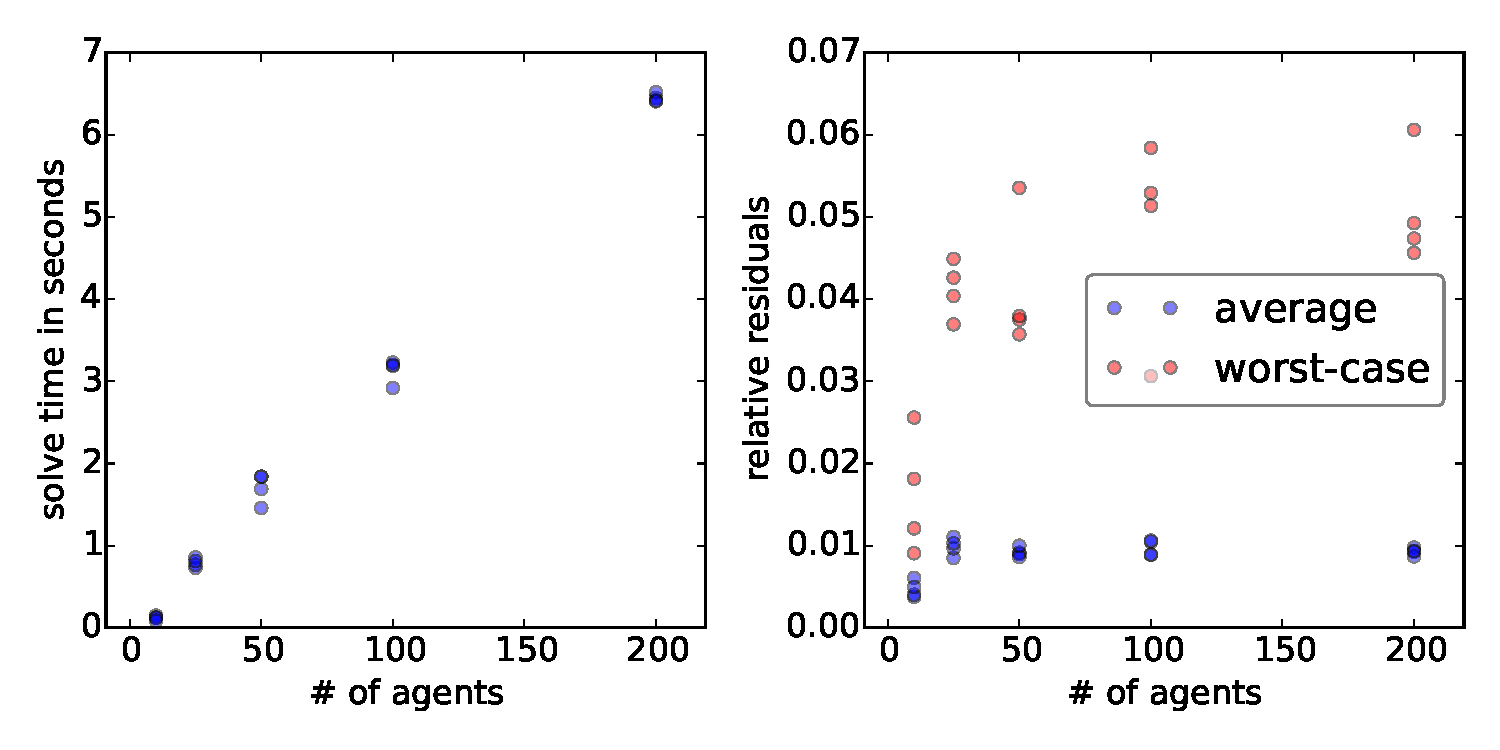
\includegraphics[width=1.0\textwidth]{figures/cvxpy}
\end{center}
\caption{XXX temporary figure.
Demonstrating the centralized algorithm of \S\ref{sec:centralized}, we give the
SCS solve times and average relative residuals of the solutions for a range of
market sizes, with 10 example markets for each size.
}
\label{f-cvxpy}
\end{figure}


\paragraph{Distributed example.}
To demonstrate the distributed algorithm of \S\ref{sec:distributed},
we solve a single random instance of size $n=10^6$ agents. At each iteration,
we take the result of the prox operation (\ref{a-prox}) and the consensus
prices $\Phi^k$ from (\ref{a-phibar}) and compute the average
relative residuals over the agents in the market and report the results in
Figure~\ref{f-admm}.

\begin{figure}
\begin{center}
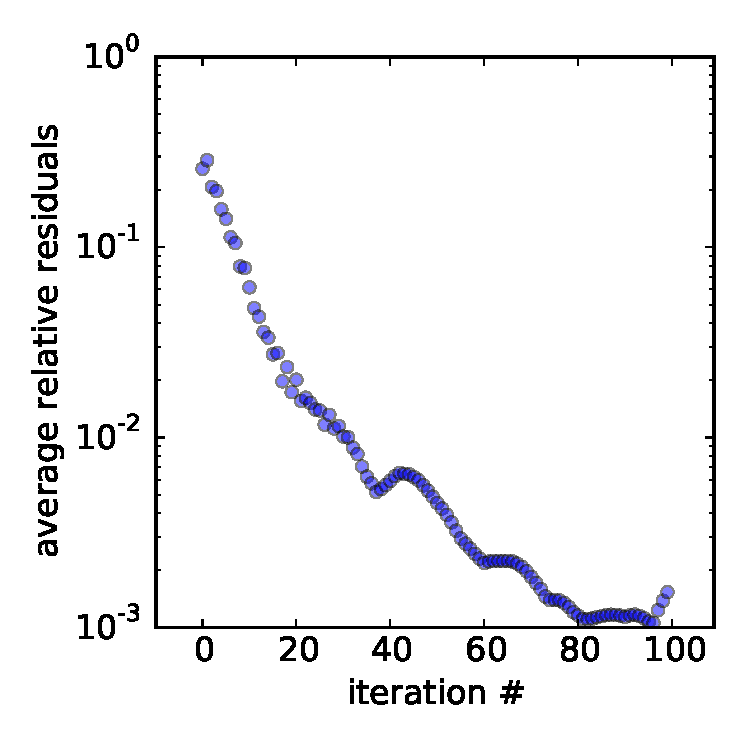
\includegraphics[width=0.6\textwidth]{figures/admm}
\end{center}
\caption{XXX temporary figure (data actually from a small example. still need
to run full-size example). This figure gives results for distributed ADMM
algorithm of \S\ref{sec:distributed} applied to a single random market
with $n=15$ agents. We report the average relative residuals as a function
of iteration number.}
\label{f-admm}
\end{figure}


\appendix


\section{Optimality conditions for exchange problem}
\label{sec:exchange_proof}

In this section, we use the same definitions and notation as in
\S\ref{sec:exchange_def}.
Consult \cite{BoV:04} as a reference for any
unfamiliar terms in this section.

The exchange UMP~(\ref{p-ump}) for an individual agent has the form
\[
\begin{array}{ll}
\mbox{minimize} & - u_i(x_i)\\
\mbox{subject to} & p^T x_i \leq p^T b_i\\
& x_i \geq 0.
\end{array}
\]

The dual of this problem is
\[
\begin{array}{ll}
\mbox{maximize} & -(- u_i)^*(\tau_i - p y_i) - p^T b_i y_i\\
\mbox{subject to} & y_i \geq 0\\
& \tau_i \geq 0,
\end{array}
\]
with $y_i \in \reals$ and $\tau_i \in \reals^n$. Here, $(- u_i)^*$
is the convex conjugate of the negative utility $-u_i$.

The Karush-Khun-Tucker (KKT) optimality conditions for agent $i$'s UMP consist
of primal feasibility, dual feasibility and zero duality gap. A solution to the
exchange MEP~(\ref{p-mep}) is given by an allocation for each agent which
satisfies that agent's UMP optimality conditions, such that the demand of the
goods does not exceed the supply. Thus, we can write the KKT conditions of the
exchange MEP as
\begin{equation}
\begin{aligned}
p y_i - \nabla u_i(x_i)&= \tau_i\\
y_i p^T x_i &= y_i p^T b_i\\
\tau_i^T x_i &= 0\\
p^T x_i &\leq p^T b_i\\
x_i, y_i, \tau_i &\geq 0\\
\sum_{i=1}^m x_{ij} &\leq \sum_{i=1}^m b_{ij},
\end{aligned}
\label{e-mep-opt1}
\end{equation}
for all $i=1,\ldots,m,\ j=1,\ldots,n$.

We can simplify the constraints by removing $\tau$:
\begin{equation}
\begin{aligned}
p y_i &\geq \nabla u_i(x_i) \\
y_i p^T x_i &= y_i p^T b_i \\
y_i p^T x_i &= \nabla u_i(x_i)^T x_i\\
p^T x_i &\leq p^T b_i\\
x_i, y_i &\geq 0\\
\sum_{i=1}^m x_{ij} &\leq \sum_{i=1}^m b_{ij}.
\end{aligned}
\label{e-mep-opt2}
\end{equation}

Next, the $y$ variables can be eliminated by combining the second and third
constraints in (\ref{e-mep-opt2}) to obtain
\[
y_i = \frac{\nabla u_i(x_i)^T x_i}{p^T b_i},
\]
which we plug it into the first constraint of (\ref{e-mep-opt2}) to get the new
set of constraints
\begin{equation}
\begin{aligned}
\frac{\nabla u_i(x_i)^T x_i}{p^T b_i} p &\geq \nabla u_i(x_i) \\
p^T x_i &\leq p^T b_i\\
x_i &\geq 0\\
\sum_{i=1}^m x_{ij} &\leq \sum_{i=1}^m b_{ij}.
\end{aligned}
\label{e-mep-opt3}
\end{equation}

The second constraint of (\ref{e-mep-opt3}) can be removed, as it is implied by
the others (which we will prove). The resulting set of constraints
\begin{equation}
\begin{aligned}
\nabla u_i(x_i)^T x_i p_j &\geq \nabla_j u_i(x_i) p^T b_i\\
\sum_{i=1}^m x_{ij} &\leq \sum_{i=1}^m b_{ij}\\
p &\geq 0\\
x_i &\geq 0,
\end{aligned}
\label{e-mep-opt4}
\end{equation}
for all $i=1,\ldots,m,\ j=1,\ldots,n$, are equivalent to (\ref{p-exchange-gp}).

\paragraph{Equivalence with original constraints.}
We have seen that conditions (\ref{e-mep-opt1}) imply conditions (\ref{e-mep-opt4}).
To see that the opposite implication holds,
multiply $x_{ij}$ with the first inequality of (\ref{e-mep-opt4}) and sum over $j$ to get
\begin{align}
&&\sum_{j=1}^n \nabla u_i(x_i)^T x_i p_j x_{ij} &\geq \sum_{j=1}^n \nabla_j u_i(x_i) x_{ij} p^T b_i \nonumber \\
&\implies & \nabla u_i(x_i)^T x_i p^T x_i &\geq \nabla u_i(x_i)^T x_i p^T b_i \nonumber\\
&\implies & p^T x_i &\geq p^T b_i. \label{e-good-ineq}
\end{align}

We see that
\begin{align*}
\sum_{i=1}^m p^T b_i &\leq \sum_{i=1}^m p^T x_i\ &&\text{(by (\ref{e-good-ineq}))}\\
&= \sum_{j=1}^n p_j \sum_{i=1}^m x_{ij} &&\\
&\leq \sum_{j=1}^n p_j \sum_{i=1}^m b_{ij}\ &&\text{(by second inequality of (\ref{e-mep-opt4}))}\\
&= \sum_{i=1}^m p^T b_i.&&
\end{align*}
This implies equality holds throughout, so, in particular,
\begin{align}
p^T x_i &= p^T b_i \label{e-spending}\\
\sum_{i=1}^m x_{ij} &= \sum_{i=1}^n b_{ij} \label{e-equilibrium}.
\end{align}

This recovers all the constraints from (\ref{e-mep-opt1}), so we see that they
are equivalent to the constraints (\ref{e-mep-opt4}).

We can interpret (\ref{e-spending}) as saying that each agent spends his entire
budget in the equilibrium solution. Constraint (\ref{e-equilibrium}) says that
there are no left-over goods at equilibrium; all goods are consumed.

\section{Other examples}

\subsection{Internet traffic routing}

A communication network is modeled as a directed graph with $m$ nodes, $n$
edges, and an edge incidence matrix $A \in \mathbf{R}^{m \times n}$, with
$A_{ij} = +1$ if edge $j$ enters node $i$, $-1$ if it exits node $i$, and 0
otherwise. Edges have latency $l \in \mathbf{R}^n_{+}$ and maximum bandwidth
$B \in \mathbf{R}^n_+$, which can be thought of as an edge capacity.

The network is shared by $r$ agents. Agent $i$ wants to maximize the throughput
between her source and sink nodes $s_i$ and $t_i$, using some fraction
of each edge's maximum bandwidth. Along a single path
between source and sink, the throughput is the minimum of the agent's usage over
each edge (but an agent may use multiple paths and chooses among all possible
paths from source to sink).

We model this as a set of
flows $F \in \mathbf{R}^{n \times r}_+$ along the edges.
Let $f_i \in \mathbf{R}^n_+$ (corresponding to the $i$th column of $F$) be the
flow of agent $i$. Flows must obey the conservation equations
$A f_i = u_i(e_{t_i} - e_{s_i})$, where $e_i \in \mathbf{R}^m$ is the standard
basis vector whose $i$th element is $1$. The total bandwidth (throughput) sent
into the sink node $t_i$ by agent $i$ is $u_i \in \reals_+$.
Note that the source and sink
nodes can send and receive unlimited bandwidth, but the flows are constrained
by the (shared) bandwidth of the edges in the network: $\sum f_i \leq B$.

The \emph{average latency} of flow $f_i$ is given by $(l^T f_i)/u_i$. Agent $i$ will
tolerate a maximum average latency $L_i$, resulting in the constraint
$l^T f_i \leq u_i L_i$.
If the network is such that no flow exists with average latency
at most $L_i$, the flow just doesn't happen: $u_i = 0$ and $f_i = 0$.

In order to allocate bandwidth to the agents in a way that accounts for their
competing interests in limited resources, we formulate a market equilibrium
problem. We price bandwidth on the edges with $p \in \mathbf{R}^n_+$, such that
the cost to agent $i$ to buy an amount $f_{ij}$ of bandwidth on edge $j$ is
given by $p_j f_{ij}$. Our goal will be to find prices $p$ so that the market
is at equilibrium. That is, agents purchasing bandwidth at prices $p$ to
maximize their throughput $u$ won't overload any edge in the network with more
bandwidth than it can handle.

Agent $i$ is given some amount of cash $w_i$ with which to purchase bandwidth
$f_i$. Acting optimally, an agent will use all of the bandwidth she purchases,
so we can equate the flow and bandwidth. The cost the agent must pay is given
by $p^T f_i$, so she is constrained by $p^T f_i \leq w_i$.

As stated, we have a Fisher equilibrium problem. Agent $i$'s utility function
over $f_i \geq 0$ is given by

$$
\begin{array}{lll}
  U_i(f_i) = &\mbox{maximize} & u_i \\
  &\mbox{subject to} & A f_i = u_i(e_{t_i} - e_{s_i})\\
  && l^T f_i \leq u_i L_i.
\end{array}
$$

Note that $U_i$ is concave, increasing, and homogeneous of degree 1, which is
what we need for the Fisher framework.

Given prices $p$, agent $i$ will solve the optimization problem

$$
\begin{array}{ll}
  \mbox{maximize} & U_i(f_i) \\
  \mbox{subject to} & p^T f_i \leq w_i \\
  & f_i \geq 0.
\end{array}
$$

To find bandwidth allocations (and prices) which solve each agent's
optimization problem and respect the total bandwidth constraints, we formulate
and solve the Fisher equilibrium problem

$$
\begin{array}{ll}
  \mbox{maximize} & \sum_i w_i\log U_i(f_i) \\
  \mbox{subject to} & \sum_i f_i \leq B\\
  & f_i \geq 0,
\end{array}
$$

which we can rewrite as

$$
\begin{array}{ll}
  \mbox{maximize} & \sum_i w_i\log u_i \\
  \mbox{subject to} & A f_i = u_i(e_{t_i} - e_{s_i})\\
  & l^T f_i \leq u_i L_i\\
  & \sum_i f_i \leq B \\
  & f_i \geq 0.
\end{array}
$$

The equilibrium allocations are given by $f_i$ and the equilbrium prices are
given as the dual variable to the constraint $\sum_i f_i \leq B$.

XXX: maybe also add the the standard Kelley example with fixed paths.


\subsection{Air-conditioning}
XXX. add market-based control of air-conditioning \cite{clearwater1996market}
control over time period. expected seasonal temps.
hourly changes. topology of air vents and/or rooms?


\subsection{multi-commodity flow}
simple generalization of the traffic flow problem?

\subsection{ad-auctions}
got to be able to come up with something

\subsection{netflix ranking}
yinuy ye's idea

\subsection{voting}
compare to alternative voting systems. quadratic voting?

\subsection{matching problem}
medical residency matching
organ donor matching

\subsection{ranking/matching}
netflix: people rank movies, movies rank people

ads: people rank ads or products, advertisers rank people (or groups of people)
based on who they want to advertise to (who they think will repsond best, or spend most)
we do this to fill user's limited adspace (budget) with ads they want to see,
while respecting advertisers budget and making everyone maximally happy.

of course, this takes in as input users utility function for content, and advertisers
utility function for users. these things might come from PCA or matrix completion.


\newpage
\bibliographystyle{alpha}
\bibliography{bibliography}

\end{document}


